\newpage
\section{Constructive heuristics}

% Introduzione
\subsection{Introduzione}
Nel (caso peggiore) di variabili binarie il livello computazionale sarà dato da $O(2^n)$ quindi il tempo di calcolo cresce esponenzialmente con il numero di variabili. 

In molte applicazioni si fa affidamento ad \hl{algoritmi detti inesatti} che \hl{CERCANO di generare delle soluzioni ammissibili}. Questi rientrano negli \hl{algoritmi euristici} dove è importante che la \hl{conoscenza del progettista venga trasmessa all'algoritmo}. Questi algoritmi possono essere:

\begin{itemize}
    \item \textbf{costruttivi}: dove \hl{cercano di generare una prima soluzione ammisibile}
    \item \textbf{migliorativi}: dove \hl{prova a migliorare la prima soluzione}
\end{itemize}

Trovare una soluzione ammissibile potrebbe essere difficile dato che potrebbe essere più complicato del trovarne una ottima.


% Travellig Salesman Problem (TSP)
\subsection{Travellig Salesman Problem (TSP)}

Data una matrice $C$ di transizione dove, per andare dal punto $1$ al $2$ \hl{pago $c_{12}$} e così via per tutte le possiabili iterazioni \hl{per un numero $n$ di punti da "visitare"}. Lo scopo sarebbe trovare un circuito che tocchi tutti i punti una sola volta con \hl{costo minimo}.

Avremo che il \hl{tempo di ciclo determina la produttivita' della macchina} tipo un robot che fa n fori e conclusi gli n fori finisce oil cilo.

Un vincolo ulteriore potrebbero essere le \hl{finestre temporali} che potrebbero esserci come nei casi di consegna dei pacchi amazon, il che \hl{rende computazionalmente piu' difficile o anche inammissibile il problema}. Notare come cambiando anche solo un dato potremmo avere una soluzione ammsisibile o una crescita esposnenziale dell'infattibilità dala quele deriva l'instabilità.


% Algoritmo greedy
\subsection{Algoritmo Greedy}

Algoritmo che \hl{cerca di massimizzare nel breve periodo} (usato per essere adattato a qualsiasi problema). È un'\hl{euristica di tipo costruttivo}, infatti ha una \hl{procedura sequenziale} che costruisce la soluzione passo passo \hl{massimizzando solo l'utilizzo immediato} andando però in contro a:

\begin{itemize}
    \item una soluzione inammissibile
    \item non garantire una soluzione ottima
\end{itemize}

il suo \hl{pseudocodice} è un adattamenteo sull'algoritmo del Travellig Salesman Problem (TSP):

\begin{itemize}
    \item[] last = 1 (last = ultimo punto toccato)
    \item[] $S = \{2,3,...,n\}$
    \item[] while ($S \neq$ insieme vuoto)
    \begin{itemize}
        \item[] estrarre da $S$ un punto
        \begin{itemize}
            \item[] $i = \text{argmin}_{i \in S} c_{\text{last}, i}$
            \item[] $\text{succ}_{last} = i$
            \item[] last $= i$
        \end{itemize}
    \end{itemize}
    \item[] $\text{succ}_{last} = 1$ 
\end{itemize}

Vediamo un esempio con dati: $n = 4$ e
$$C=
\left[ {\begin{array}{cccc}
    0 & 10 & 5 & 8 \\
    10 & 0 & 2 & 1 \\
    5 & 2 & 0 & 4 \\
    8 & 1 & 4 & 0 \\
\end{array} } \right]
$$

dove applicando l'algoritmo abbiamo:

\begin{itemize}
    \item last = 1; $\rho = <2,3,4>$
    \item last = 3 ; $\rho=<2,4>$; $\text{succ}_1 = 3$
    \item last = 2; $\rho=<4>$; $\text{succ}_3 = 2$
    \item last = 4; $\rho =<>$; $\text{succ}_2 =4$
    \item $\text{succ}_4 = 1$
\end{itemize}


% Miller-Tucker-Zemlin
\subsection{Miller-Tucker-Zemlin}

Questo modello definisce delle \hl{variabili binare $x_{ij}$} per ogni coppia di punti $i$ e $j$:

$$ x_{ij} =
\begin{cases} 
    1, \text{ se } i,\ j \text{ sono/saranno visitati} \\ 
    0, \text{altrimenti}
\end{cases}
$$

avremo allora che:
$$\min \sum_{i,j} c_{i,j} x_{i,j}$$
s.t
\begin{itemize}
    \item $\sum{j} x_{ij} = 1\ \ \ \forall i$
    \item $\sum{j} x_{ji} = 1\ \ \ \forall i\ ->$ dice che ogni punto ha un suo successore
    \item $0 \leq x_{ij} \leq 1\ \ \ \forall x_{ij} \text{ integer} ->$ dice ogni punto ha un predecessore
\end{itemize}

Questi \hl{vincoli non bastano} per poter risolvere il modello, infatti non possiamo escludere di avere una \hl{soluzione disconnessa (sub-tour)}


\begin{figure}[H]
\centering
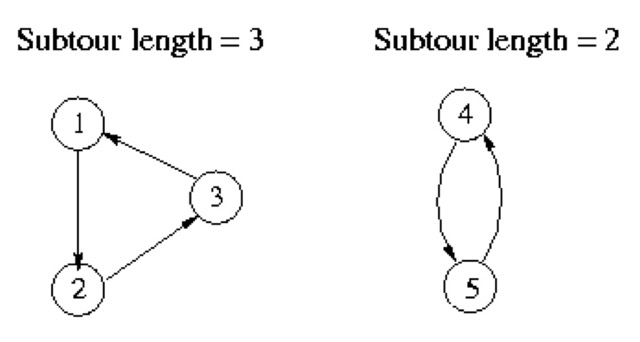
\includegraphics[scale=0.3]{sep.jpeg}
\caption{Soluzione disconnessa} 
\label{sep}
\end{figure}


Si introducono allora dei \hl{vincoli di connessione} della soluzione tramite una \hl{variabile per l'ordine di vista: $u_i$} (una per ogni punto).

Poniamo allora un punto iniziale con $u_i = 1$:

\begin{itemize}
    \item[] $u_1 = 1 -> x_{1,3} = 1$
    \item[] $u_3 = 2 -> x_{3,4} = 1$
    \item[] $u_4 = 3 -> x_{4,2} = 1$
    \item[] $u_2 = 4 -> x_{2,1} = 1$
\end{itemize}

altri \hl{vincoli da imporre su $u_i$}:

\begin{itemize}
    \item $2 \leq u_i \leq 1\ \ \ \forall i \neq 1$
    \item $u_i - u_j + 1 <= n(1-x_{ij})\ \ \ \forall i,j \neq 1$
\end{itemize}

Avremo quidni \hl{2 casi}:

\begin{itemize}
    \item $x_{ij} = 0\ \Rightarrow\ u_i - u_j +1 \leq n$: ovvio dato che tutte le variabili \textbf{$u$ sono comprese in $n$}
    \item $x_{ij} = 1\ \Rightarrow\ u_i - u_j + 1 \leq 0$: dato che $u_j \geq u_i + 1$ allora \textbf{$i$ predecessore di $j$}
\end{itemize}


% Algoritmo relax-and-fix
\subsection{Algoritmo relax-and-fix}

Si usa per \hl{problemi multiperiodali} dato che voglio poter avere un approccio con \hl{suddivisione in piu' periodi temporali}:

$$\min z = c^Tx$$
s.a.
\begin{itemize}
    \item $Ax=b$
    \item $x \geq 0$ (integer)
\end{itemize}

\hl{Partiziono le variabli in $n$ gruppi} in modo da avere variabili impiegate per un solo intervallo di tempo. Allora il problema diventa:

abbiamo alloradelle applicazioni ndove le varaibili naturalemte si dividono in gruppi datoun osviluppo temporale, il orblema allora diventa:

$$\min z = \sum_{i=1}^n c_i^Tx_i$$
s.a.
\begin{itemize}
    \item $\sum_{i=1}^na_ix_i=b$
    \item $x_i \geq 0$ (integer)
\end{itemize}

la difficoltà del problema si trova nelle molte varibili intere. Posso allora \hl{definire un problema con variaibli $x_1$ del primo gurppo intere}, per le restanti faccio un rilassamento. Potremo avere che:


\begin{itemize}
    \item ausiliario: inammissibile $\to$ iniziale: inammissibile
    \item ausiliario: sol. ottima $\to$ fisso $x_1$ alla soluzione: $x_1 = \overline{x}_1$
\end{itemize}

Quindi per \hl{risolvere il problema} dobbiamo:

\begin{enumerate}
    \item $\underline{x}_1$ diventa \textbf{intera}
    \begin{itemize}
        \item \textbf{rilasso} le altre variabili
        \item \textbf{risolvo} il problema e \textbf{fissiamo} $x_1 = \overline{x}_1$ che viene "rimossa" dal modello
    \end{itemize}

    \item ecc, ecc...
\end{enumerate}

Così facendo \hl{tengo conto delle variabili "future"} senza richiede un grande sforzo computazione, dato che lavora sul singolo gruppo.

\hl{Generallizzando}:
$$\min x = \sum_{i=1}^{k-1} c_i \overline{x}_i + c_k x_k + \sum_{i=k+1}^n c_i x+i$$
s.t

\begin{itemize}
    \item $\sum_{i=1}^{k-1} a_i \overline{x}_i + a+k x+k + \sum_{i=k+1}^n a_i x_i = b$
    \item $x_k \geq 0$ (integer)
    \item $x_i \geq 0$
\end{itemize}

Lo \hl{pseudocodice} sarà:

\begin{itemize}
    \item[] found = true
    \item[] for (k = 1 $\to$ n):
    \begin{itemize}
        \item[] solve $P_k(\overline{x}_1,...,\overline{x}_{k-1})$
        \item[] if è inammissibile:
        \begin{itemize}
            \item[] found = false
            \item[] break;
        \end{itemize}
        \item[] else: $(x'_{k+1},...,x'_n)$ è soluzione
        fissare $\overline{x}_k = x'_{k}$
    \end{itemize}
\end{itemize}


% Algoritmo rolling horizon
\subsection{Algoritmo rolling horizon}

Durante il primo periodo considero di:

\begin{enumerate}
    \item creare un \hl{sottoproblema con alcune variabili} da $x_1$ a $x_k$
    \item \hl{trascurare le variabili dei periodi successivi}
    \item fisso $x_1$
    \item mi \hl{muovo di uno step}
    \item considero un \hl{sottoproblema con $x_1$}
    \item \hl{fisso $x_2$} e considero le variabili fino a $x_k+1$.
    \item ecc, ecc...
\end{enumerate}

Andiamo quindi a \hl{risolvere un problema a $k$ variabili} ma \hl{senza tenere in conto le variabili troppo successive}, quindi sarà meno accurato.


% Multiple criteria decision making
\subsection{Multiple criteria decision making}

Spesso abbiamo \hl{piu' obbiettivi} e \hl{non riusciamo a scegliere in anticipo quale ha priorita'} allora spesso vanno in \hl{conflitto}, allora cerchiamo di trovare le migliori soluzioni che devono \hl{rispettare alcuni vincoli}:

$$p \text{ criteria } =
\begin{cases} 
    z_1 = f_1(x) \text{ da }\min \text{ o }\max \\ 
    z_2 = f_2(x) \text{ da }\min \text{ o }\max \\ 
    ... \\
    z_p = f_p(x) \text{ da }\min \text{ o }\max
\end{cases}
$$
s.t

\begin{itemize}
    \item $g(x) \geq 0$
    \item $x \geq 0$
\end{itemize}


% Esempio problema scheduling
\subsection{Esempio problema scheduling}

Preso un problema di scheduling, abbiamo $n$ attività con paramentri:

\begin{itemize}
    \item $S_i$: starting time dell'attività $i$
    \item $d_i$: durata dell'attività $i$
    \item $p_{ij} = 1$ se l'attivtà $j$ è prerequinistito dell'attività $i$
    \item $p_{ij} = 0$ altrimenti
\end{itemize}

come f.o: $\min T$ con $T$ tempo di completamento:
$$\min T$$
s.t.

\begin{itemize}
    \item $T \geq S_i + d_i,\ i = 1, ..., n$
    \item $S_i \geq p_{ij} (S_j + d_j),\ i,j = 1, ..., n$
\end{itemize}

Per poter \hl{formulare un'attivita' in modo fattibile}:

\begin{itemize}
    \item $D_i$: max durata dell'attività $i$
    \item $b_i$: min durata dell'attività $i$
    \item $d_i$: durata dell'attività $i$
    \item $X_i$: costo per accellerare il completamento dell'attività $i$
\end{itemize}


allora:

\begin{itemize}
    \item $d_i = D_i-a_iX_i$ con $a_i$ coefficente in unità di tempo
    \item $d_i \geq b_i$
\end{itemize}

abbiamo da minimizzare 2 obiettivi:
$$min \sum_{i=1}^n X_i$$
$$min T$$
s.t.

\begin{itemize}
    \item $T \geq S_i + d_i\ \ \ \forall\ \ \ i$
    \item $S_i \geq p_{ij} (S_j + d_j)\ \ \ \forall\ \ \ i, j, i \neq j$
    \item $d_i \geq b_i\ \ \ \forall\ \ \ i$
    \item $d_i = D_i - a_i X_i\ \ \ \forall\ \ \ i$
\end{itemize}


% Superior solutions
\subsection{Superior solutions}

Preson un problema con \hl{piu' obiettivi} allora ne consideriamo uno con obiettivo singolo, allora \hl{rappresento i singoli obiettivi} nello spazio.

Presa una soluzione potremo trovarne una migliore ma solo \hl{se si trova nella zona ammissibile e che sia nella frontiera}, in caso contrario è detta \hl{utopia}.

\begin{figure}[H]
\centering
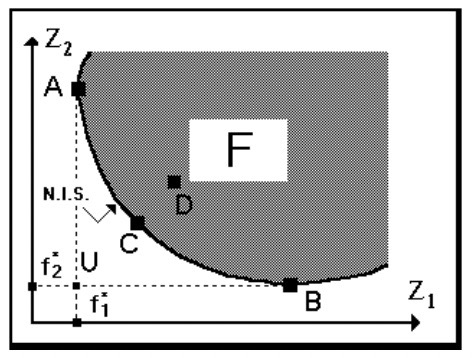
\includegraphics[scale=0.3]{utop.jpeg}
\caption{Utopia} 
\label{utop}
\end{figure}

Definiamo invece \hl{soluzione superiore} la soluzione che minimizza o massimizza meglio di tutte (come U se fosse nella zona ammissibile).

Si parla allora di soluzioni dominate e soluzioni non dominate (di \hl{Pareto}).

Per \hl{confrontare due soluzioni di Pareto} usiamo il \hl{trade-off ratio} tamite:

$$|\frac{z_i(x_A)-z_i(x_B)}{z_j(x_A)-z_j(x_B)}|$$

che rappresenta il \hl{miglioramento dell'obiettivo i-esimo in base al miglioramento di un altro obiettivo}.

Nel caso di una \hl{zona convessa} collegneremo i punti limite tramite una \hl{tangente immagginaria}, dalla quale però non prendere mo i punti di frontiera.

\begin{figure}[H]
\centering
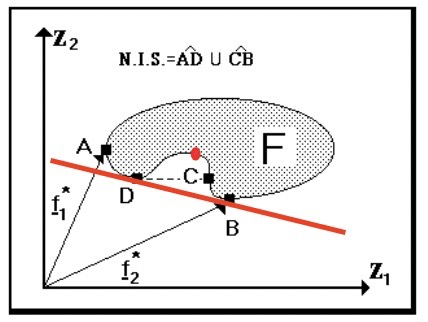
\includegraphics[scale=0.3]{convess.jpeg}
\caption{Zona convessa} 
\label{convess}
\end{figure}

per \hl{trovare le soluzioni efficenti} abbiamo 2 metodi:

\begin{enumerate}
    \item \hl{metodo dei vincoli}: \textbf{considero un solo obiettivo}, per gli altri avrò:
        $$\min f_i(x)$$
        
        s.t
        
        \begin{itemize}
            \item $f_k(x) \leq u_k$
            \item $g(x) \geq 0$
            \item $x \geq 0$
        \end{itemize}

        Prendo allora solo $A$ e $D$:

        \begin{figure}[H]
        \centering
        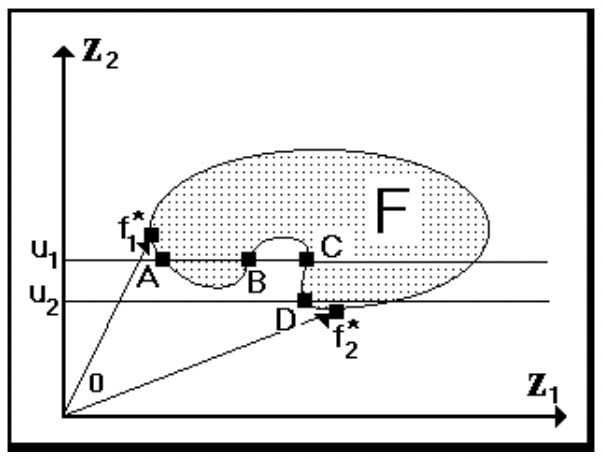
\includegraphics[scale=0.3]{vinc.jpeg}
        \caption{Metodo dei vincoli} 
        \label{vinc}
        \end{figure} 
    \item \hl{metodo dei pesi}: abbiamo una sola \textbf{f.o somma di tutti li obiettivi}:
        $$\min \sum_{i=1}^p w_i f_i (x)$$

        s.t
        
        \begin{itemize}
            \item $\sum_{i=1}^p w_i = 1$
            \item $g(x) \geq 0$
            \item $x \geq 0$
            \item $w_i \geq 0$
        \end{itemize}

        \begin{figure}[H]
        \centering
        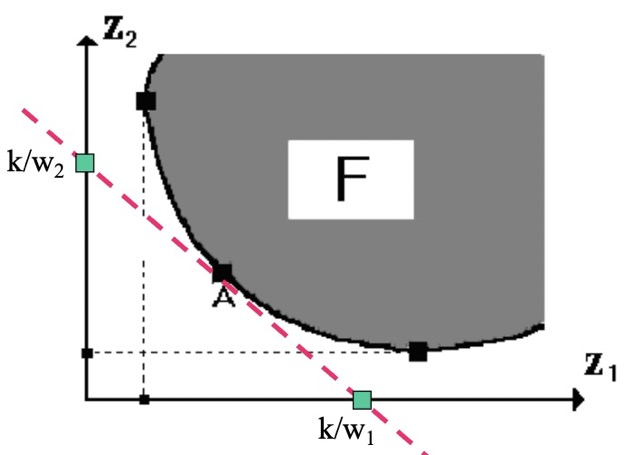
\includegraphics[scale=0.3]{pesi.jpeg}
        \caption{Metodo dei pesi} 
        \label{pesi}
        \end{figure}

        dove a seconda del valore che diamo ai pesi andiamo a \hl{spostare la retta trangente alla zona ammissibile}.
\end{enumerate}


% Metodo a priori
\subsection{Metodo a priori}

Per \hl{risolvere il singolo problema} usiamo:
$$\max U(f_1(x), f_2(x), ..., f_p(x))$$

s.t
\begin{itemize}
    \item $g(x) \geq 0$
    \item $x \geq 0$
\end{itemize}

ma in genere \hl{non si trova} questa soluzione.


% Metodo a posteriori
\subsection{Metodo a posteriori}

Generiamo tutte le \hl{soluzioni efficienti per dire quale e' la migliore}. Notare che così facendo si potrebbe avere una \hl{crescita esponenziale} del problema.

Una buona \hl{alternativa} è il metodo interattivo.


% Metodo interattivo
\subsection{Metodo interattivo}

Presi 2 obiettivi:

\begin{itemize}
    \item troviamo il \hl{punto ottimo per entrambi}
    \item troviamo la \hl{prima soluzione efficiente che sia tra $A$ e $C$}
    \item scegliere su \hl{quale parte della frontiera posizionarsi}
    \item ecc, ecc...
\end{itemize}

\begin{figure}[H]
\centering
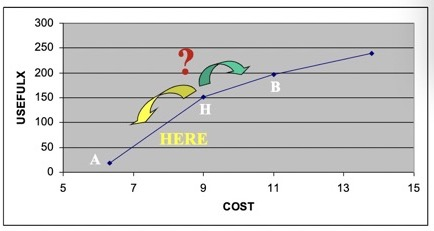
\includegraphics[scale=0.5]{intent.jpeg}
\caption{Metodo interattivo} 
\label{intent}
\end{figure}

mi fermerò quando il segmento che rimane è \hl{cosi piccolo che i due punti conincidono}.
